% Pregunta 2:

Considera la siguiente gram\'atica donde $A$ es el s\'imbolo inicial:
\[
\begin{array}{rcl}
A & \to & bB \\
B & \to & cC \\
B & \to & cCe \\
C & \to & dA\\
A & \to & a\\
\end{array}
\]
\begin{enumerate}

    \item \textbf{(1pt.)} Describe formalmente el lenguaje que acepta la gram\'atica.\\

        Sea $L$ el lenguaje que acepta la gramatica anterior\\
        $L = (\{A,B,C\}, \{a,b,c,d,e\}, P, A)$\\
        $P = \{A & \to & bB, B & \to & cC, B & \to & cCe, C & \to & dA, A & \to & a\}$\\

    \item \textbf{(3pts.)} Proporciona el aut\'omata para construir la tabla de parsing \textbf{LR(1)}.

        \begin{center}
            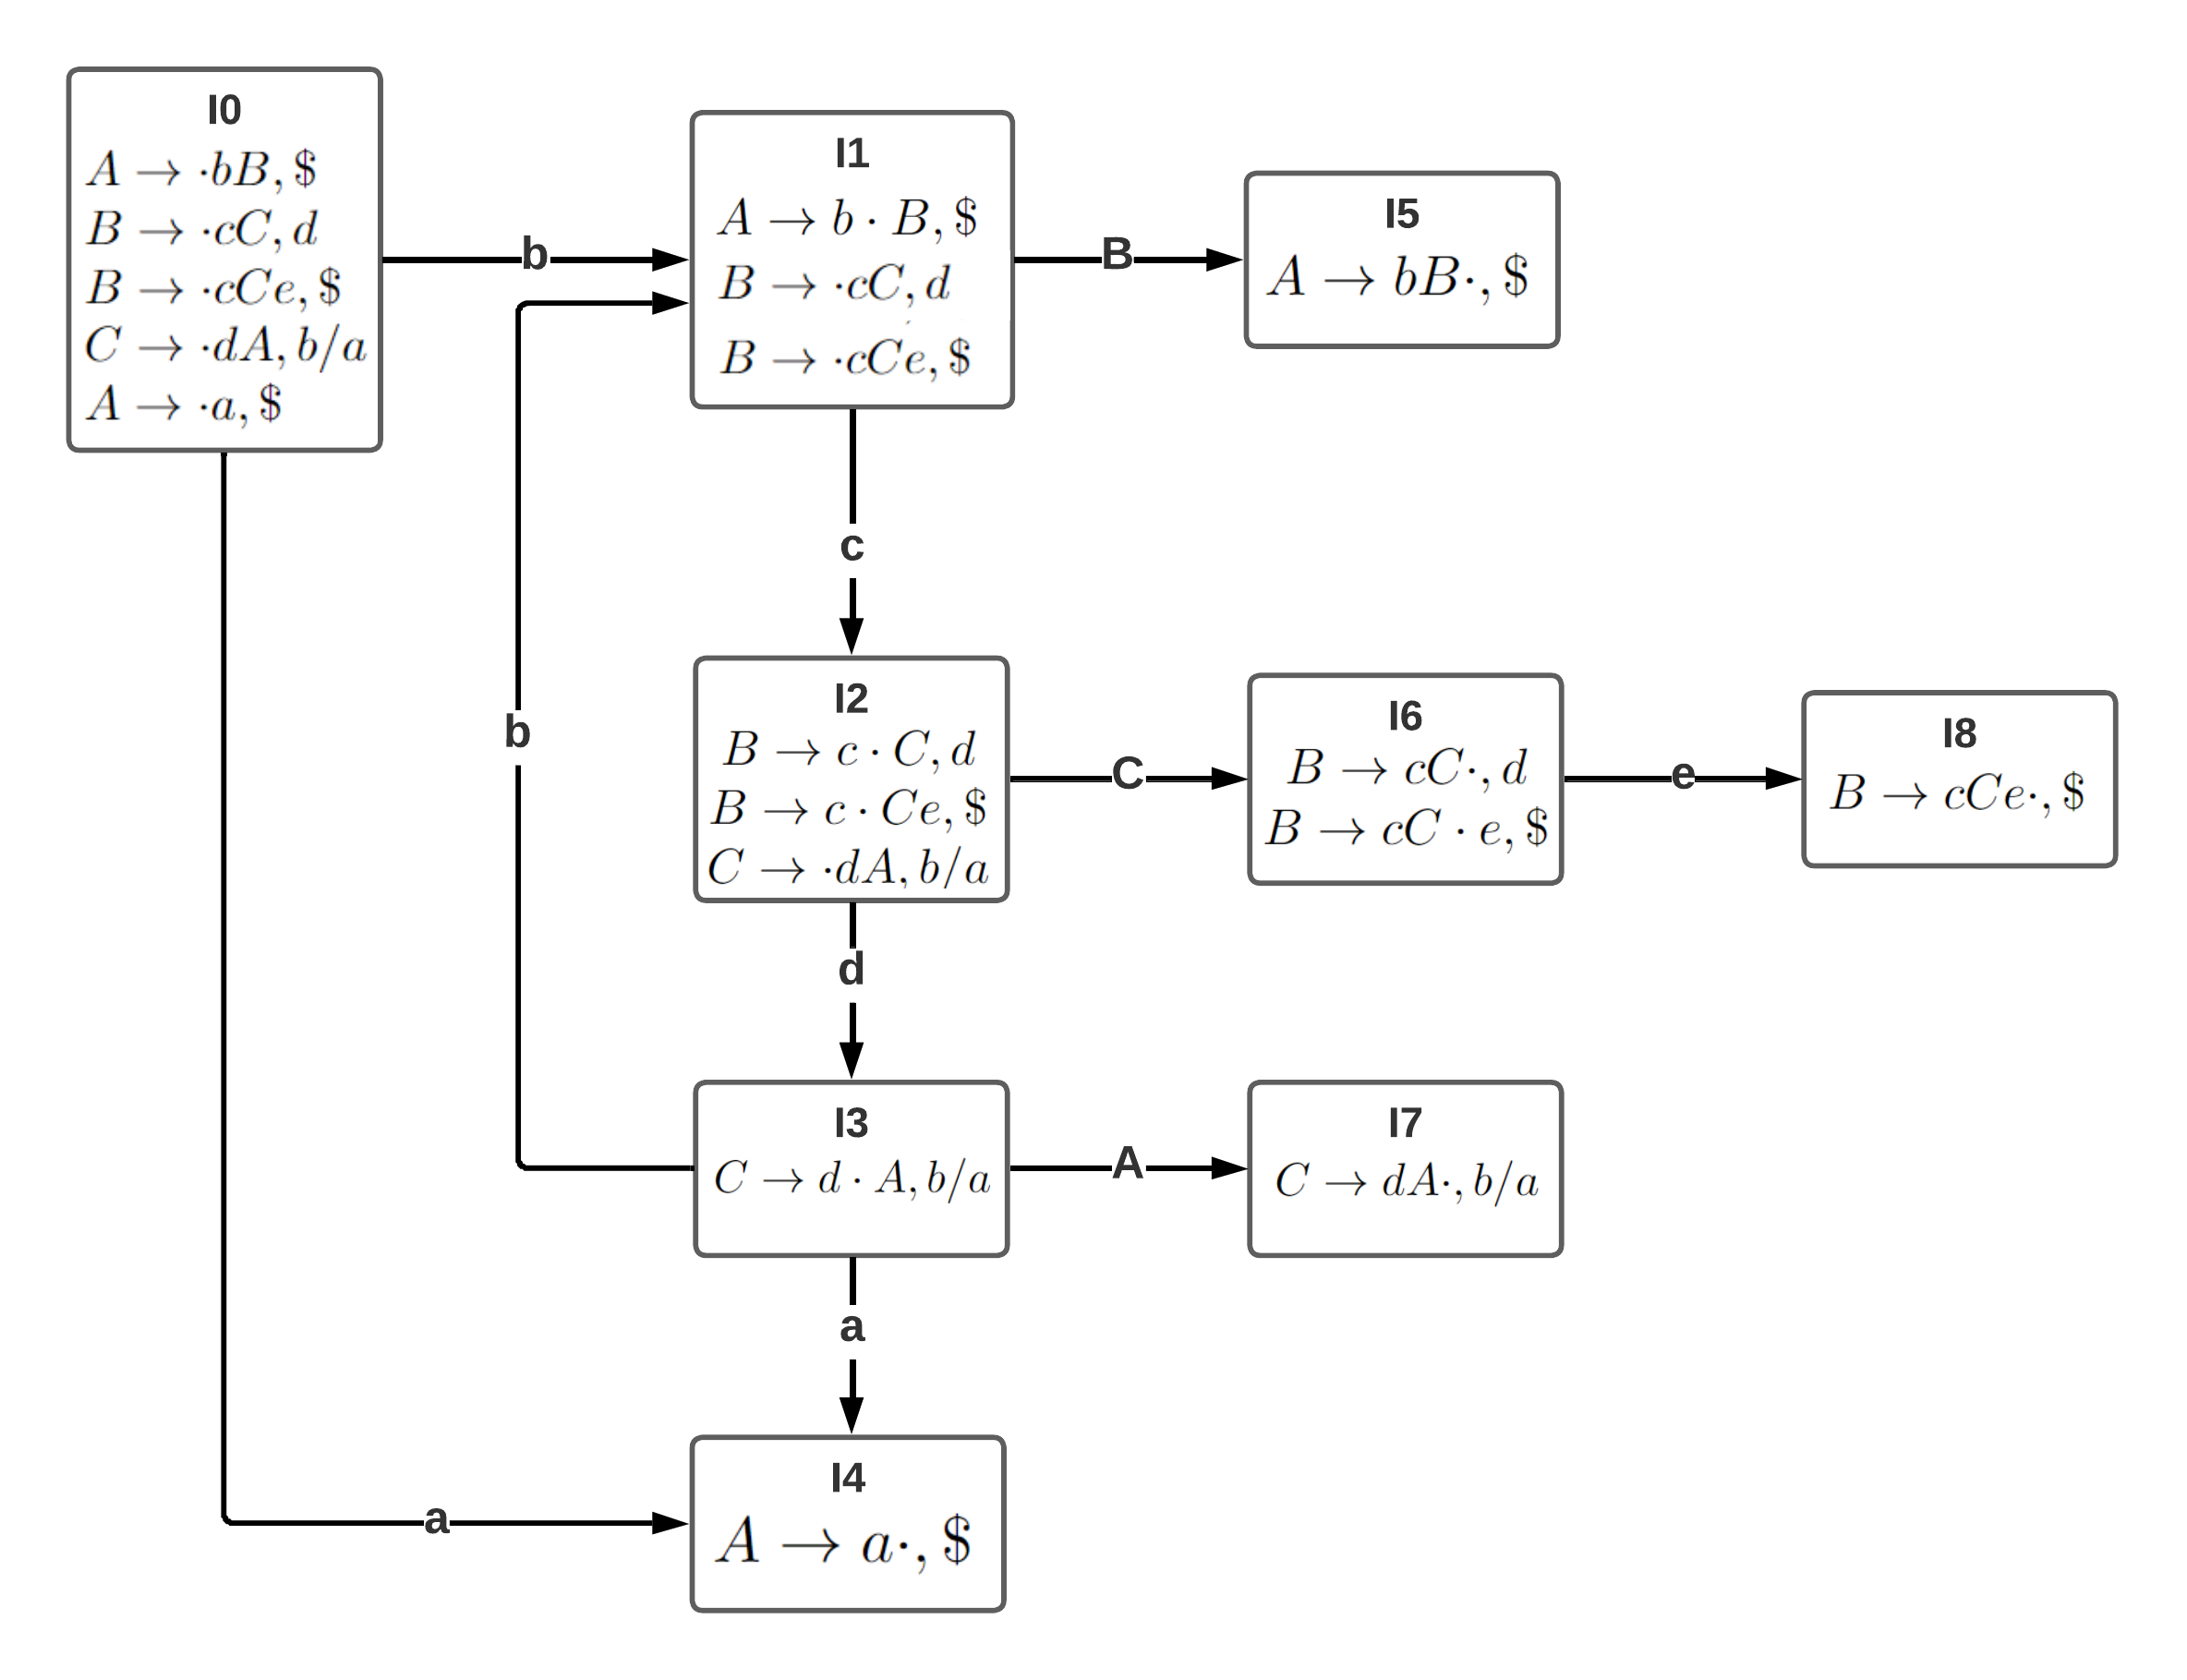
\includegraphics[scale = 0.65]{../Imagen/T4_Ej2b}
        \end{center}

        Debido a que hay un conflicto en la transición de $C \rightarrow dA$ no es posible que sea LR\\

    \item \textbf{(1pt.)} De ser posible, analiza una cadena no trivial y de longitud
    al menos 4, mostrando la secuencia de acciones del aut\'omata mediante una tabla
    que incluya al menos la actualizaci\'on de la cadena de entrada y la actualizaci\'on
    de la pila.\\

        Cadena : $bcdae$

        \begin{table}[h]
            \centering
            \caption{Tabla del progreso del automata}
            \label{tab:3.2}
            \begin{tabular}{|l|r|l|}

                \hline
                Pila del Parser & Cadena & Regla aplicada \\
                \hline
                \$A & $bcdae\$$ & \\
                \hline
                \$Bb & $bcdae\$$ & $A \to bB$ \\
                \hline
                \$B & $cdae\$$ & \\
                \hline
                \$eCc & $cdae\$$ & $B \to cCe$ \\
                \hline
                \$eC & $dae\$$ & \\
                \hline
                \$eAd & $dae\$$ & $C \to dA$ \\
                \hline
                \$eA & $ae\$$ & \\
                \hline
                \$ea & $ae\$$ & $A \to a$ \\
                \hline
                \$e & $e\$$ & \\
                \hline
                \$ & $\$$ & \\
                \hline
                \$ & \$ & ACEPTADA \\
                \hline

            \end{tabular}
        \end{table}

\end{enumerate}